\chapter{Da semente à planta}\label{ch:g2:from-seed-to-plant}

Sacuda uma vagem seca de feijão e caem feijõezinhos duros --- secos,
sem graça, aparentemente tão sem vida quanto cascalho. Mas plante um
deles na terra e regue: em poucos dias acontece algo extraordinário
debaixo do chão. Uma \omterm{def:g1:plants-around-us:plant}{planta} inteira estava dobrada lá dentro,
esperando o sinal dela.

\section{O que é uma semente}

\begin{definition}[Semente]\label{def:g2:from-seed-to-plant:seed}
Uma \emph{semente}\index{semente} é o começo de uma \omterm{def:g1:plants-around-us:plant}{planta} nova,
feita pela planta-mãe. Dentro da casca que a protege, a semente
guarda:
\begin{itemize}
  \item uma plantinha já começada --- o \emph{germe}\index{germe (da
        semente)} da \omterm{def:g1:plants-around-us:plant}{planta}, com o início de uma \omterm{def:g1:plants-around-us:parts}{raiz} e de um broto;
  \item uma reserva de alimento para alimentar essa plantinha até
        ela conseguir se alimentar sozinha.
\end{itemize}
\end{definition}

\begin{example}[Abrindo um feijão de molho]\label{ex:g2:from-seed-to-plant:open}
Deixe um feijão branco grande de molho de um dia para o outro e a
casca sai fácil. O feijão se abre em duas metades gordinhas --- a
reserva de alimento --- e ali, encaixadinha numa das bordas, está
uma plantinha clara, com a ponta da \omterm{def:g1:plants-around-us:parts}{raiz} e as primeiras \omterm{def:g1:plants-around-us:parts}{folhas}
dobradas, pequena como um grão de arroz. A \omterm{def:g1:plants-around-us:plant}{planta} nova estava lá o
tempo todo.
\end{example}

\begin{omfigure}
\begin{tikzpicture}
  \node[anchor=south west, inner sep=0] (img) at (0,0)
    {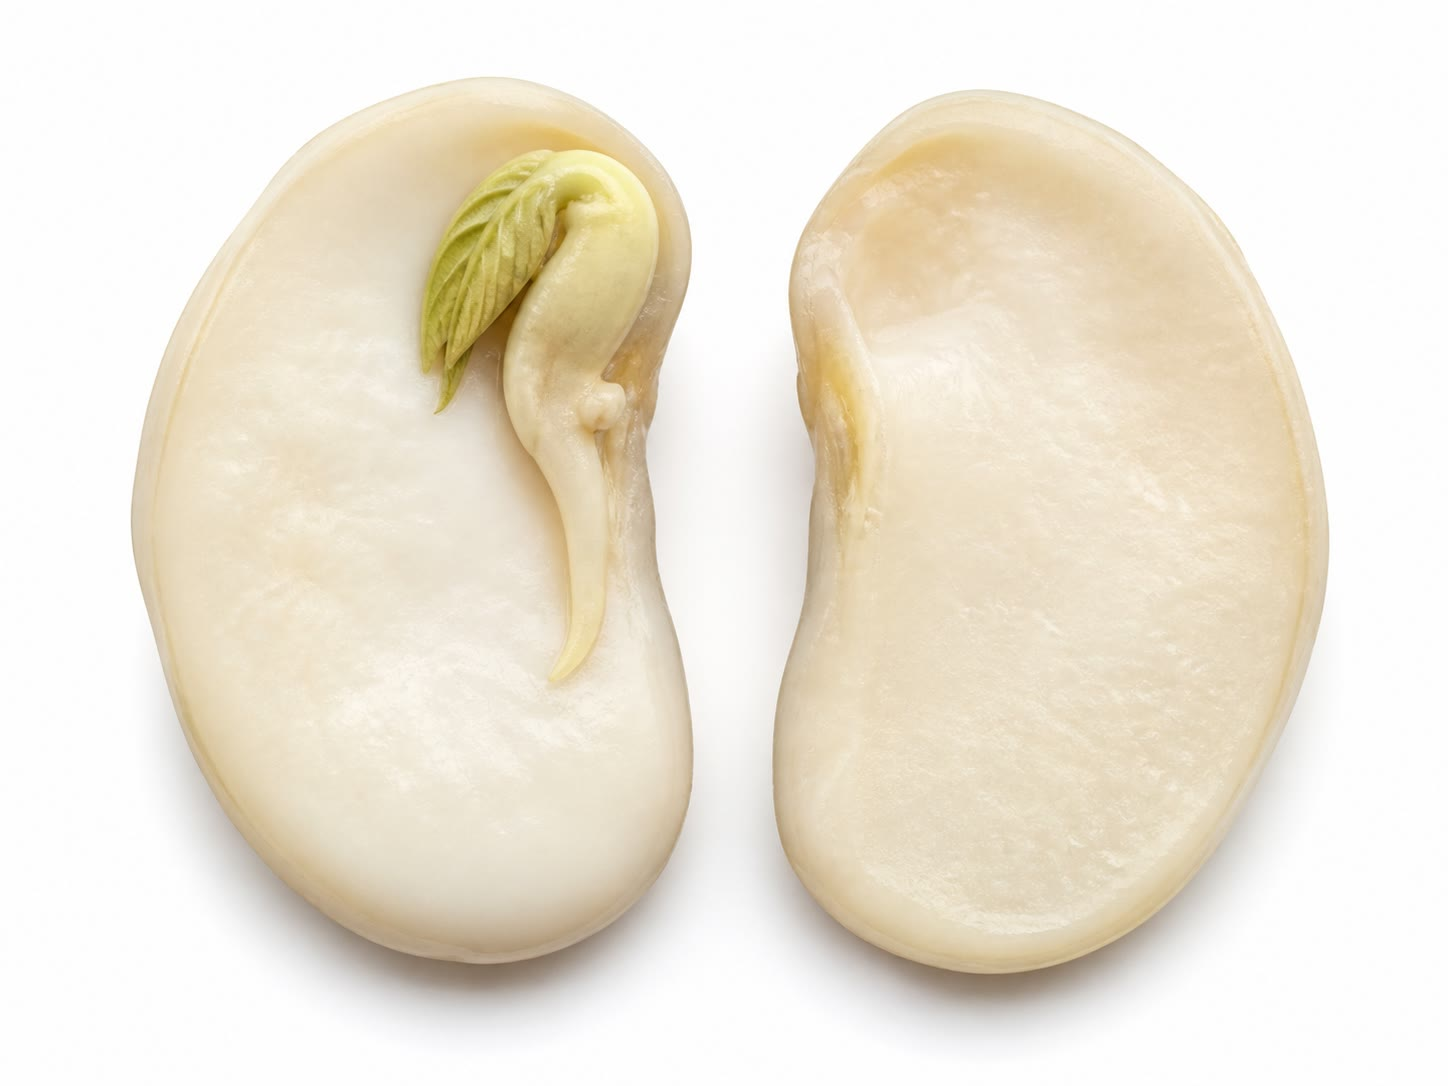
\includegraphics[width=0.62\linewidth]{images/book1/ai/fig-bean-open.jpg}};
  \begin{scope}[x={(img.south east)}, y={(img.north west)},
      every node/.style={font=\small}]
    \draw[omDef, thick] (0.35,0.79) -- (0.26,0.94)
      node[above] {as primeiras folhas dobradas};
    \draw[omDef, thick] (0.40,0.38) -- (0.28,-0.04)
      node[below] {a ponta da raiz};
    \draw[omDef, thick] (0.78,0.35) -- (0.80,-0.04)
      node[below, align=center] {as duas metades gordinhas:\\ a reserva de alimento};
  \end{scope}
\end{tikzpicture}

{\small Dentro do feijão de molho e aberto: uma plantinha --- ponta
da \omterm{def:g1:plants-around-us:parts}{raiz} e primeiras \omterm{def:g1:plants-around-us:parts}{folhas} dobradas --- encostada na reserva de
alimento.}
\end{omfigure}

\begin{remark}[As sementes passam pela nossa cozinha]\label{rem:g2:from-seed-to-plant:kitchen}
Feijão, ervilha, lentilha, arroz, \omterm{def:g2:from-seed-to-plant:seed}{semente} de girassol, os caroços da
maçã e o caroço do pêssego: a cozinha é cheia de \omterm{def:g2:from-seed-to-plant:seed}{sementes}. Algumas
são minúsculas, como a \omterm{def:g2:from-seed-to-plant:seed}{semente} de papoula; o coco é uma gigante.
Cada uma delas, se tivesse chance, tentaria virar uma \omterm{def:g1:plants-around-us:plant}{planta}.
\end{remark}

\section{Germinação}

\begin{definition}[Germinação]\label{def:g2:from-seed-to-plant:germination}
\emph{Germinação}\index{germinação} é o momento em que a \omterm{def:g2:from-seed-to-plant:seed}{semente}
acorda e começa a crescer: ela incha com a água, a casca se abre, a
raizinha sai primeiro e mergulha para baixo, depois o broto sobe,
levando as primeiras \omterm{def:g1:plants-around-us:parts}{folhas} verdes na direção da luz. Dizemos que a
\omterm{def:g2:from-seed-to-plant:seed}{semente} \emph{germina}\index{germinar}.
\end{definition}

\begin{proposition}[Do que uma semente precisa para germinar]\label{prop:g2:from-seed-to-plant:needs}
Para \omterm{def:g2:from-seed-to-plant:germination}{germinar}, uma \omterm{def:g2:from-seed-to-plant:seed}{semente} precisa de \emph{água} e de
\emph{calor}. Ela ainda não precisa de luz: a reserva de alimento
alimenta a plantinha no começo, mesmo debaixo da terra, no escuro.
Sem água, ou no frio, uma \omterm{def:g2:from-seed-to-plant:seed}{semente} boa simplesmente espera.
\end{proposition}
\admitted

\begin{example}[Por que se planta na primavera]\label{ex:g2:from-seed-to-plant:spring}
Quem cuida da horta \omterm{def:g1:plants-around-us:plant}{planta} feijão na primavera, e não no inverno: a
\omterm{def:g2:from-seed-to-plant:seed}{semente} na terra fria ficaria esperando --- ou apodreceria --- em vez
de \omterm{def:g2:from-seed-to-plant:germination}{germinar}. Dias quentes e terra regada são exatamente os dois
sinais da \cref{prop:g2:from-seed-to-plant:needs}.
\end{example}

\begin{method}[Plantar uma semente e ver a germinação]\label{met:g2:from-seed-to-plant:sow}
\begin{enumerate}
  \item Forre um vidro com algodão ou papel úmido;
  \item escorregue um feijão entre o vidro e o algodão, para você
        conseguir enxergar;
  \item deixe o vidro num cômodo quentinho e o algodão úmido;
  \item olhe todo dia e anote o que vê: o feijão inchando, a casca
        se abrindo, a \omterm{def:g1:plants-around-us:parts}{raiz} para baixo, o broto para cima.
\end{enumerate}
O vidro deixa visível o que normalmente acontece debaixo da terra.
\end{method}

\begin{omfigure}
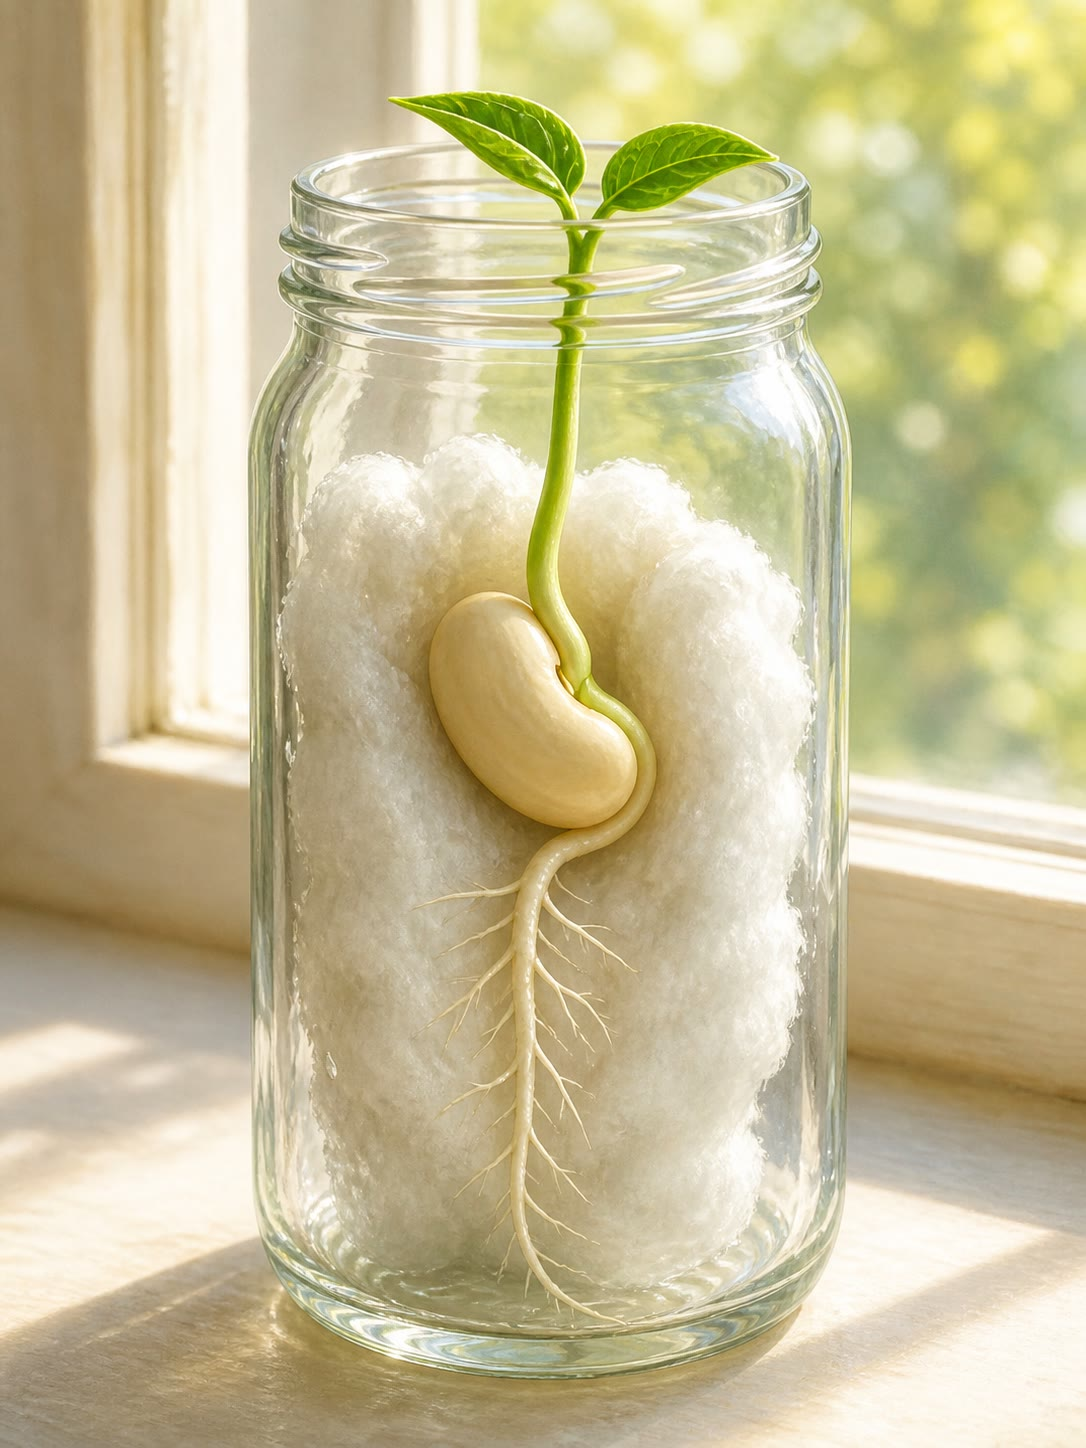
\includegraphics[width=0.44\linewidth]{images/book1/ai/g2-seed-bean-jar.jpg}

{\small A experiência do vidro no meio da \omterm{def:g2:from-seed-to-plant:germination}{germinação}: \omterm{def:g1:plants-around-us:parts}{raiz} para
baixo, broto para cima e a \omterm{def:g2:from-seed-to-plant:seed}{semente} se esvaziando entre os dois.}
\end{omfigure}

\begin{remark}[Raiz para baixo, broto para cima --- sempre]\label{rem:g2:from-seed-to-plant:updown}
Não importa como o feijão fique no vidro --- de lado, de cabeça para
baixo ---, a \omterm{def:g1:plants-around-us:parts}{raiz} sempre se vira para baixo e o broto sempre se vira
para cima. A plantinha não enxerga e, mesmo assim, sabe para que
lado é em cima. As \omterm{def:g1:plants-around-us:plant}{plantas} percebem mais do que mostram.
\end{remark}

\section{Da plantinha à planta com sementes}

\begin{proposition}[O ciclo de vida da planta]\label{prop:g2:from-seed-to-plant:cycle}
A \emph{plântula}\index{plântula} vira uma \omterm{def:g1:plants-around-us:plant}{planta} com \omterm{def:g1:plants-around-us:parts}{raízes}, \omterm{def:g1:plants-around-us:parts}{caule}
e \omterm{def:g1:plants-around-us:parts}{folhas}; a \omterm{def:g1:plants-around-us:plant}{planta} dá \omterm{def:g1:plants-around-us:parts}{flores}; as \omterm{def:g1:plants-around-us:parts}{flores} fazem novas
\emph{\omterm{def:g2:from-seed-to-plant:seed}{sementes}}; e o ciclo pode recomeçar. Um único pé de feijão
pode fazer dezenas de feijões novos num só verão.
\end{proposition}
\admitted

\begin{example}[Um feijão, um verão]\label{ex:g2:from-seed-to-plant:summer}
Plantado em maio, um feijão \omterm{def:g2:from-seed-to-plant:germination}{germina} em uma semana; em junho já é uma
\omterm{def:g1:plants-around-us:plant}{planta} cheia de \omterm{def:g1:plants-around-us:parts}{folhas} subindo pela estaca; em julho vêm as \omterm{def:g1:plants-around-us:parts}{flores}
brancas, depois as vagens verdes; em agosto as vagens pendem
pesadas, cada uma com uma fileira de feijões novos --- as \omterm{def:g2:from-seed-to-plant:seed}{sementes} do
ano que vem, feitas pela \omterm{def:g1:plants-around-us:plant}{planta} deste ano.
\end{example}

\section{Exercícios}

\begin{exercise}[$\star$]\label{exo:g2:from-seed-to-plant:1}
Que duas coisas ficam dentro da casca de uma \omterm{def:g2:from-seed-to-plant:seed}{semente}?
\end{exercise}

\begin{exercise}[$\star$]\label{exo:g2:from-seed-to-plant:2}
O que quer dizer \emph{\omterm{def:g2:from-seed-to-plant:germination}{germinar}}? O que sai primeiro da \omterm{def:g2:from-seed-to-plant:seed}{semente}: a
\omterm{def:g1:plants-around-us:parts}{raiz} ou o broto?
\end{exercise}

\begin{exercise}[$\star$]\label{exo:g2:from-seed-to-plant:3}
Diga as duas coisas de que uma \omterm{def:g2:from-seed-to-plant:seed}{semente} precisa para \omterm{def:g2:from-seed-to-plant:germination}{germinar}. Qual
necessidade famosa das \omterm{def:g1:plants-around-us:plant}{plantas} crescidas \emph{não} está na lista?
\end{exercise}

\begin{exercise}[$\star$]\label{exo:g2:from-seed-to-plant:4}
Como uma plantinha enterrada consegue crescer no escuro, antes de
chegar à luz? De onde vem o alimento dela no começo?
\end{exercise}

\begin{exercise}[$\star$]\label{exo:g2:from-seed-to-plant:5}
Diga quatro \omterm{def:g2:from-seed-to-plant:seed}{sementes} que você poderia encontrar numa cozinha.
\end{exercise}

\begin{exercise}[$\star$]\label{exo:g2:from-seed-to-plant:6}
Por que se \omterm{def:g1:plants-around-us:plant}{planta} na primavera em vez do inverno?
\end{exercise}

\begin{exercise}[$\star$]\label{exo:g2:from-seed-to-plant:7}
Ponha em ordem: vagem com feijões novos --- \omterm{def:g2:from-seed-to-plant:seed}{semente} --- \omterm{def:g1:plants-around-us:plant}{planta} com
\omterm{def:g1:plants-around-us:parts}{flores} --- \omterm{prop:g2:from-seed-to-plant:cycle}{plântula} --- \omterm{def:g1:plants-around-us:plant}{planta} cheia de \omterm{def:g1:plants-around-us:parts}{folhas}.
\end{exercise}

\begin{exercise}[$\star$]\label{exo:g2:from-seed-to-plant:8}
Faça a experiência: monte o vidro do
\cref{met:g2:from-seed-to-plant:sow} com dois feijões --- um deitado
de lado, outro de cabeça para baixo. Depois da \omterm{def:g2:from-seed-to-plant:germination}{germinação}, compare
as \omterm{def:g1:plants-around-us:parts}{raízes} e os brotos. O que a \cref{rem:g2:from-seed-to-plant:updown}
prevê?
\end{exercise}

\begin{exercise}[$\star\star$]\label{exo:g2:from-seed-to-plant:9}
A Nina guarda um pacote de \omterm{def:g2:from-seed-to-plant:seed}{sementes} de feijão numa gaveta seca
durante um ano inteiro, e elas ainda germinam quando ela finalmente
\omterm{def:g1:plants-around-us:plant}{planta}. Por que elas não cresceram nem morreram na gaveta? Use a
\cref{prop:g2:from-seed-to-plant:needs}.
\end{exercise}

\begin{exercise}[$\star\star$]\label{exo:g2:from-seed-to-plant:10}
O pintinho do \cref{ch:g2:animals-grow-up} cresce dentro do \omterm{def:g2:animals-grow-up:born}{ovo},
alimentado pela gema. O que faz o papel da gema dentro de um feijão?
O que um \omterm{def:g2:animals-grow-up:born}{ovo} e uma \omterm{def:g2:from-seed-to-plant:seed}{semente} têm em comum?
\end{exercise}
